%
% Latex Document made by TheInevitables for Architecture Requirements etc,  COS 301 2017
%


\documentclass{article}

\usepackage{geometry}
\usepackage[utf8]{inputenc}
\usepackage{graphicx}
\usepackage{float}
\usepackage{amsmath}
\usepackage{amsfonts}
\usepackage{amssymb}
\usepackage{graphicx}
\usepackage{float}


\DeclareGraphicsExtensions{.png}
\DeclareGraphicsExtensions{.jpg}
\graphicspath{ {Diagrams/} }

 \geometry{
 a4paper, 
 total={170mm, 257mm}, 
 left=25mm, 
right=25mm, 
 top=25mm, 
 }
 
 \title{ Software Requirements Specification \\ COS-301 \\ The Inevitables \\[0.5cm] 
\includegraphics[width=6cm]{front-page}}
 
 \author{Drew Langley \hfill 11039753 \\ Lyle Nel \hfill 29562695 \\ Dawie Pritchard \hfill 13104340 \\  Peter Rayner \hfill [Student Number]\\ Rian van der Merwe \hfill 15101283 }
\date{23 May 2017}

%%%%%%%%%%%%%%%%%%%%%%%%%%%%%%%%%%%%%%%%%%%%%%%%%%%%%%%%%%%%%%%%%%%%%%%%%%%%%%%%%
%%%%%%%%%%%%%%%%%%%%%%%%%%%%%%%%     START     %%%%%%%%%%%%%%%%%%%%%%%%%%%%%%%%%%%%%%%%%%%
%%%%%%%%%%%%%%%%%%%%%%%%%%%%%%%%%%%%%%%%%%%%%%%%%%%%%%%%%%%%%%%%%%%%%%%%%%%%%%%%%
\begin{document}
\maketitle
\pagebreak
\tableofcontents
\pagebreak

\section{External Interface Requirements}
    \subsection{User Interfaces}
        The mobile application will interface with the supported input and output
        features of the host's operating system. Inputs include text that the user
        will enter for login or searching a venue. Outputs include the type of fonts
        to display text or graphics to show images or draw the map.

    \subsection{Hardware Interfaces}
        Since neither the mobile application nor the web portal have any designated
        hardware, it does not have any direct hardware interfaces. The WiFi software
        in the mobile phone manages the built-in WiFi and the hardware connection
        to the database server is managed by the underlying operating system on the
        mobile phone and the web server.

    \subsection{Software Interfaces}
        The mobile application communicates with the WiFi software in order to get
        signal strength information from multiple WiFi access points to determine
        (using triangulation) where the user is located. The communication software
        between the database and mobile application consists of operation concerning
        creating, reading, removing and modifying the data.

    \subsection{Communication Interfaces}
        The communication between the different parts of the system are important since they depend on each other. However, in what way the communication is achieved is not important for the system and is therefore handled by the underlying operating systems for both the mobile application and the back-end of the system.

\section{Performance Requirements}
\input{performance_req}
\newpage
\section{Design Constraints}
\input{design_con}
\newpage
\section{System Software Attributes}

    \subsection{Reliability}

        \begin{description}

        \item[$\bullet$] Any information that is stored on the database must remain correct when being transferred to the user interface.
        \item[$\bullet$] The services offered by the system should be available to users except for when the system is undergoing maintenance.
        \item[$\bullet$] The system should reply to user requests in the shortest time interval possible.
        \item[$\bullet$] The system must be fault tolerant, it needs to maintain a certain level of performance and offer other services that are not affected by this fault to the users.
        \item[$\bullet$] In the event of a fault the system must be able to recover within the shortest time period possible and recover any data that may have been lost.
        \item[$\bullet$] The system should be able to respond appropriately if it receives bad input data from the user.

        \end{description}

    \subsection{Scalability}

        \begin{description}

        \item[$\bullet$] The system must be able to cater for increases in the work load, for example large number of users or activities at any given time, without impacting the performance of the system.
        \item[$\bullet$] If the system does not cater for increases in workload it should at least provide the ability to be readily enlarged.

        \end{description}

    \subsection{Maintainability}

        \begin{description}

        \item[$\bullet$] The system must be designed in a modular fashion that provides high cohesion and loose coupling, this will allow parts of the system to be easily maintained without affecting the rest of the system.
        \item[$\bullet$]Maintenance should be able to be carried out by different maintenance teams, therefore the system must be easy to learn and understand.

        \end{description}

    \subsection{Integrability}

        \begin{description}

        \item[$\bullet$] Since we are following a modular design, components of the system that are separately developed should work correctly together.
        \item[$\bullet$] Follow coding standards specified by the client to allow for easy integration and employ continuous integration in our design process.

        \end{description}

    \subsection{Usability}

        \begin{description}

        \item[$\bullet$] The system must be easy to learn.
        \item[$\bullet$]System must cater for user mistakes, by providing the user with the undo or roll back options.
        \item[$\bullet$]The user interface must be easy to use and must be intuitive.
        \item[$\bullet$]The system should display options in a logical manner.
        \item[$\bullet$]Incorporate widgets and icons that the target users may be familiar with.
        \item[$\bullet$]The user manual should have a detailed description of the system.
        \item[$\bullet$]A help option must be provided to the users.

        \end{description}

    \subsection{Interoperability}

        \begin{description}

        \item[$\bullet$]The system must be able to communicate with the University of Pretoria WiFi system, because the WiFi  access points will be used for the navigation.

        \end{description}
\newpage
\section{Modules}

	\subsection{Overview of System}
	\input{overview}
	\newpage
    \subsection{User Management}
        \subsubsection{Class Diagram}
        		\begin{figure}[H]
  			\caption{Users Class Diagram}
  			\centering
    			\includegraphics[height=12cm]{UsersClassDiagram}
		\end{figure}
		\newpage
        \subsubsection{Activity Diagrams}
        	\begin{figure}[H]
  			\caption{Activity Diagram - Log In}
  			\centering
    			\includegraphics[width=8cm]{ActivityDiagram-LogIn}
		\end{figure}

		\begin{figure}[H]
  			\caption{Activity Diagram - Register}
  			\centering
    			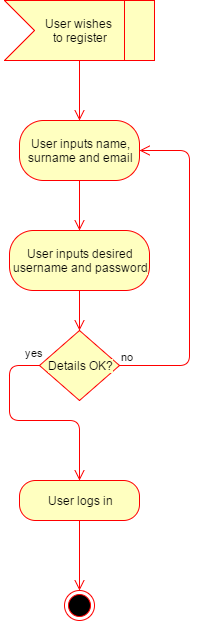
\includegraphics[height=15cm]{ActivityDiagram-Register}
		\end{figure}

		\begin{figure}[H]
  			\caption{Activity Diagram - Administrators}
  			\centering
    			\includegraphics[height=15cm]{ActivityDiagram-Admin}
		\end{figure}

		\newpage
        \subsubsection{State Diagram}
        	\begin{figure}[H]
  			\caption{State Diagram - User Management}
  			\centering
    			\includegraphics[width=15cm]{StateDiagram-UserManagement}
		\end{figure}
        %\subsubsection{Chosen Design Patterns}
	\newpage
    \subsection{Notifications}
        \subsubsection{Class Diagram}
		\begin{figure}[H]
  			\caption{Notifications Class Diagram}
  			\centering
    			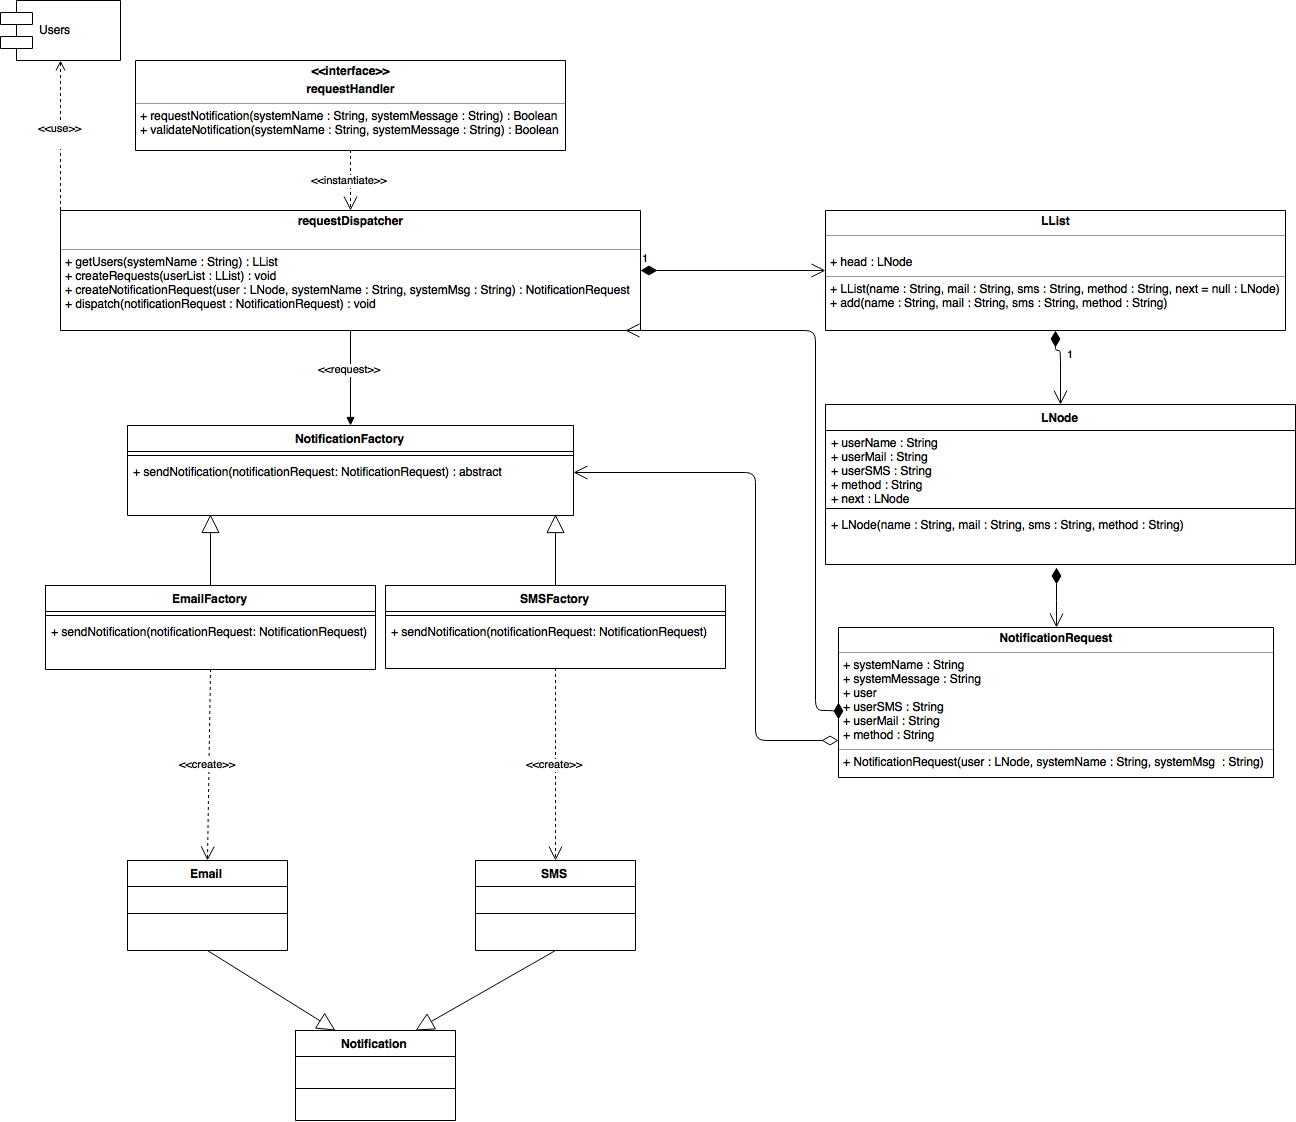
\includegraphics[width=\textwidth]{Notifications_Class_Diagram}
		\end{figure}
        \subsubsection{Use Case Diagrams}
		\begin{figure}[H]
  			\caption{Notifications Use Case Diagram}
  			\centering
    			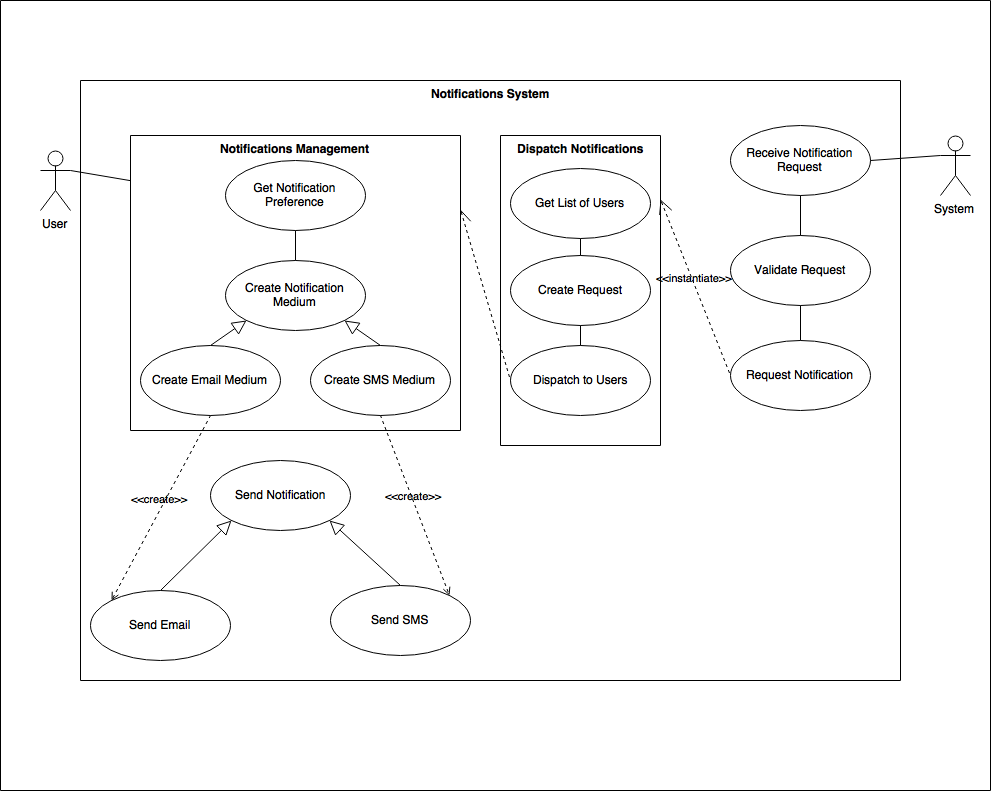
\includegraphics[width=\textwidth]{NotificationUseCases}
		\end{figure}
        \subsubsection{Chosen Design Patterns}

        We have chosen to incorporate the Factory Design Pattern in our design of the notifications module for NavUP. Due to the fact that notifications are generated and then sent to the respective mediums, it makes sense to implement the above pattern for the following reasons:
		\begin{description}

		\item[$\bullet$]Extendibility : Should NavUP need to facilitate a greater range of mediums to communicate system updates, and entire re-code of the module would not be necessary.

		\item[$\bullet$]Ease-of-use : The notifications management interface need not know what class of the object it is creating, instead leaving it up to the respective child classes to decide. This abstraction makes life easier for programmers to use the module.

		\item[$\bullet$]Modularity : Having the factory become an interface for sending through various mediums, creates a somewhat modular approach within the subsystem.
		\end{description}
    \newpage

    \subsection{Navigation}
        \subsubsection{Class Diagram}
        \begin{figure}[H]
        	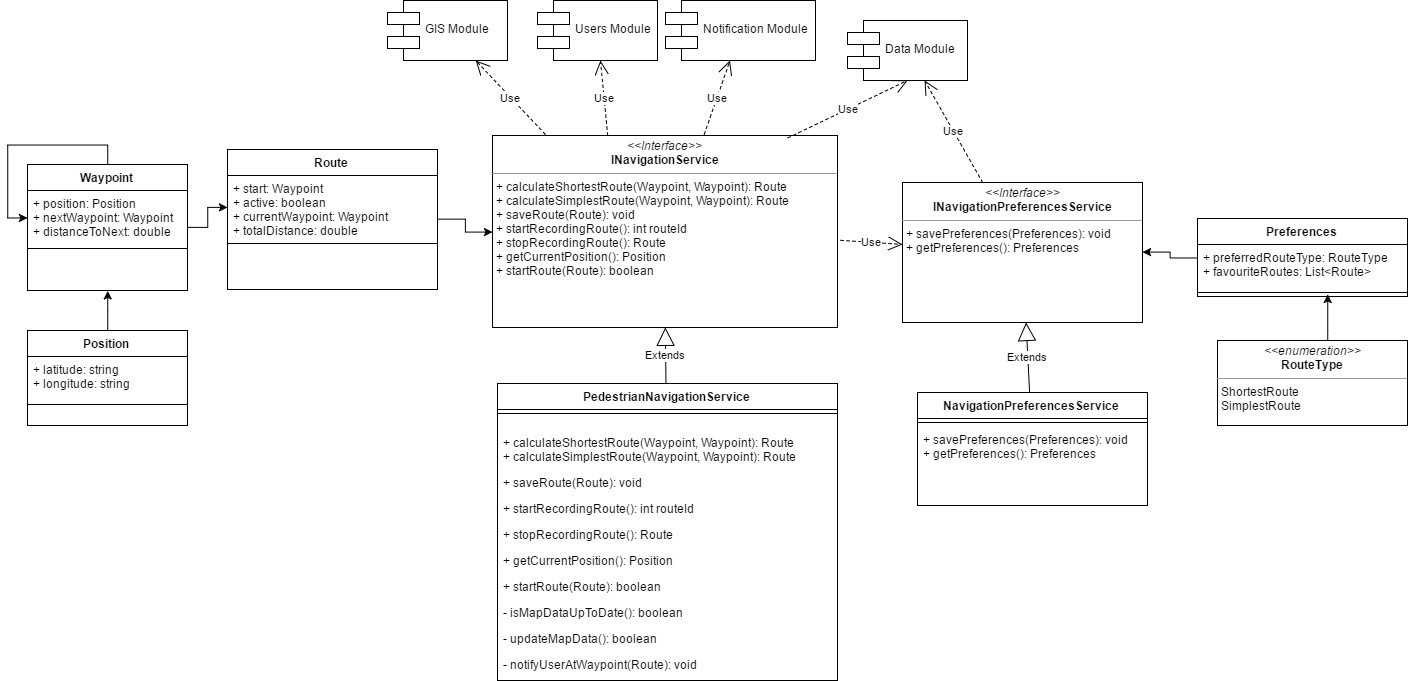
\includegraphics[width=\textwidth]{Navigation_Class_Diagram}
            \caption{Navigation Module Class Diagram}
        \end{figure}
        \subsubsection{Use Case Diagrams}
        \begin{figure}[H]
        	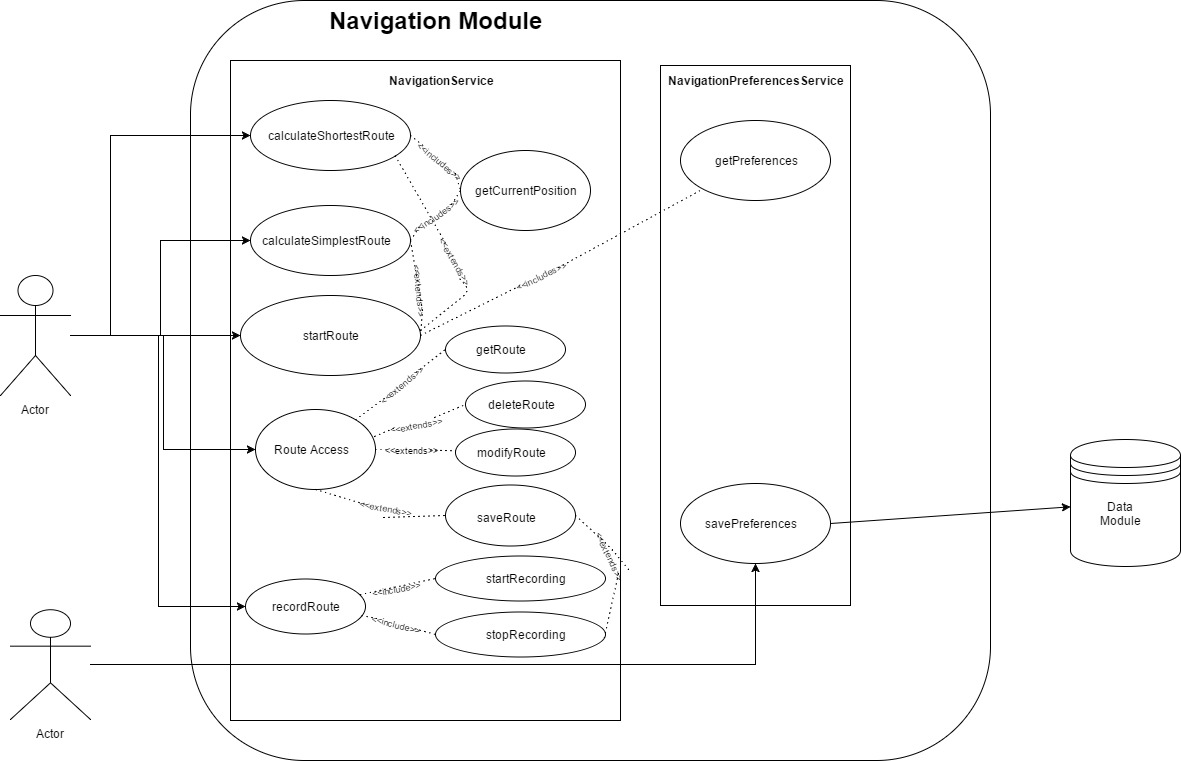
\includegraphics[width=\textwidth]{Navigation_Use_Case_Diagram}
            \caption{Navigation Module Use Case Diagram}
        \end{figure}
        \subsubsection{Other Diagrams}

        \begin{figure}[H]
        	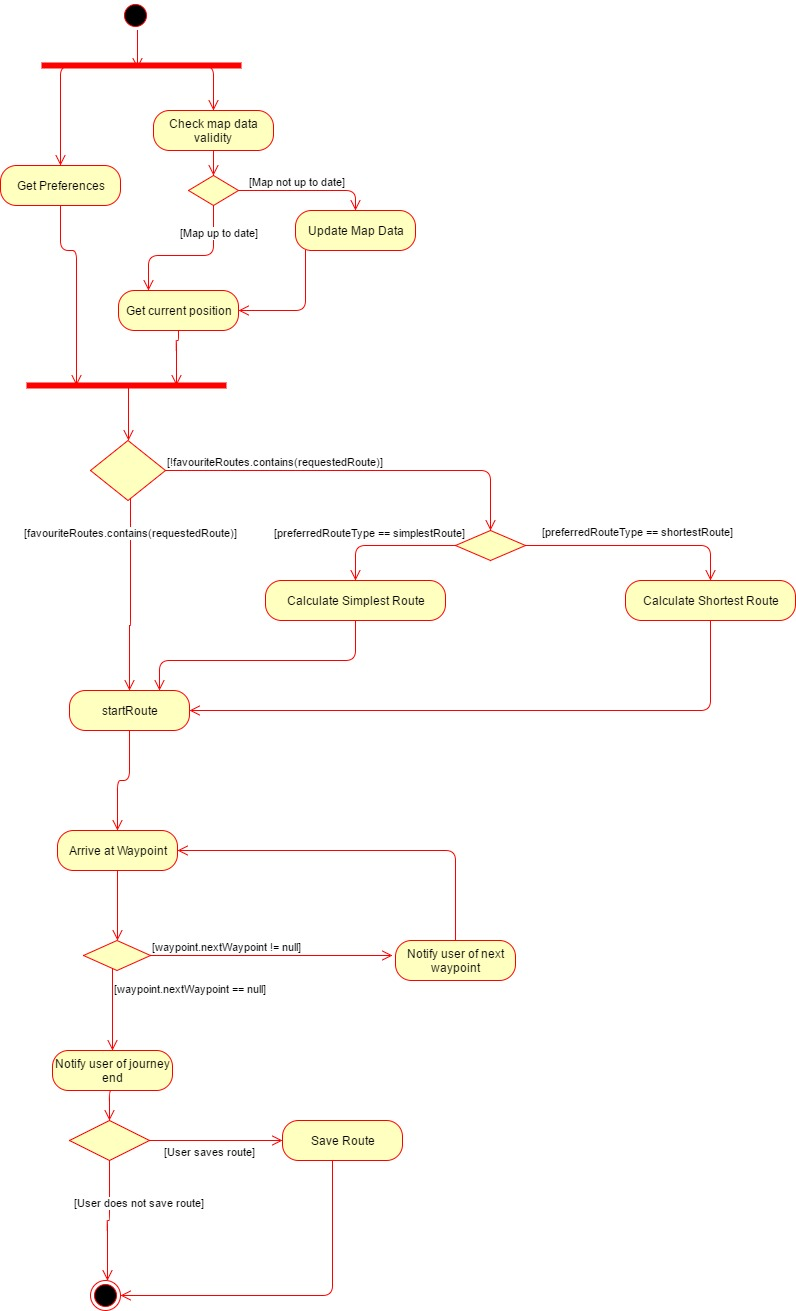
\includegraphics[width=\textwidth]{Navigation_Activity_Diagram}
        	\caption{Navigation Module Activity Diagram}
        \end{figure}
        \newpage

    \subsection{Points-of-interest}

        \subsubsection{Class Diagram}

	  \begin{figure}[H]
            \centering
            \includegraphics[width = \textwidth, height = 15cm ]{new_points_of_interest_class_diagram}
            \caption{Points of Interest Class Diagram}
            \label{Points of Interest Class Diagram}
        \end{figure}

        \subsubsection{Use Case Diagram}

	 \begin{figure}[H]
            \centering
            \includegraphics[width = \textwidth, height = 15cm ]{points_of_interest_use_case_diagram}
            \caption{Points of Interest Use Case Diagram}
            \label{Points of Interest Use Case Diagram}
        \end{figure}

        \subsubsection{Chosen Design Patterns}

	 For the Points of Interest Class Diagram the Factory and Facade design patterns are used. The Facade design pattern provides a unified interface to a set of interfaces in the Points of Interest subsystem. The Facade defines a higher-level interface for the Points of Interest that makes the subsystem easier to use. Thus it wraps a complicated subsystem with a simpler interface. The Factory design pattern provides an interface for creating families of related or dependent objects without specifying their concrete classes.

\newpage
\section{Technology Choices}
\input{technology}

\end{document}
